\scanpage{94}
\[
\begin{aligned}
\underline{\mathrm{H}}^{\unsure{11|1,1}}(A\times_S B)&=\underline{\mathrm{H}}^{\unsure{11|1,1}}(A/S)\oplus\underline{\mathrm{H}}^{\unsure{11|1,1}}(B/S)\\
&\quad+\underline{\mathrm{H}}^{1,0}(A/S)\otimes\underline{\mathrm{H}}^{0,1}(B/S)+\underline{\mathrm{H}}^{0,1}(A/S)\otimes\underline{\mathrm{H}}^{1,0}(B/S)
\end{aligned}
\]
La classe $\xi$ qu'on veut calculer a, pour des raisons de fonctorialité (regarder les inclusions $A\longrightarrow A\times_S B$, $B\unsure{\longrightarrow|{-}}A\times_S B$) des composantes nulles sur les deux premiers facteurs. Il reste à calculer sa classe dans les derniers, on trouve ce qu'on \unsure{pense}\ldots

\figure{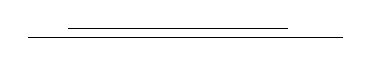
\begin{tikzpicture}\draw (0,0)--(4,0);\draw (.5,.12)--(3.3,.12);\end{tikzpicture}}

\deleted{Connexion \inserted{(absolue)} canonique sur $\underline{M}_{X/S}$}

\deleted{$\underline{W}_{X'_1/S'}\simeq\underline{W}_{X'_2/S'}$ canoniquement ??}

\margin{\diagram{\begin{tikzcd}[column sep=small,row sep=small]
\deleted{X_0} \arrow[r,dash]\arrow[d,dash] & \deleted{\unsure{X'_1}} \arrow[d,dash] & \deleted{\unsure{X''_2}} \arrow[dl,dash] \\
\deleted{S_0} \arrow[r,phantom,"\deleted{\subset}"] & \deleted{\unsure{S'|S''}} &
\end{tikzcd}}
\deleted{dans le voisinage inf. du premier ordre de $S$ avec $\exists$ rétraction de $S$ sur $S_0$}}

\deleted{\uline{Question équivalente}. Si on a un $L_0$ inversible sur $X_0$, muni d'une connexion rel. à $S_0$, alors les \unsure{prolongts} (avec connexions) à $X'$ et à $X''$ se correspondent \unsure{biunivoquement}.}

\margin{$\unsure{W_{X/S}}$}
\margin{$S_0\longleftarrow S$}
\margin{93}
